\documentclass[border=4pt]{standalone}
\usepackage{tikz}
\usetikzlibrary{arrows,arrows.spaced,positioning}
\begin{document}
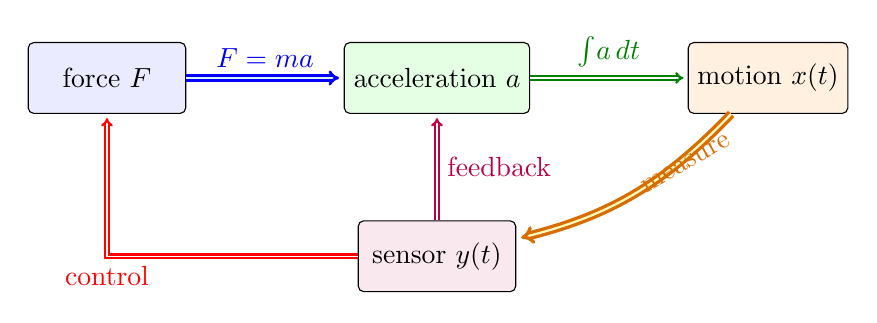
\begin{tikzpicture}[
  node distance=1.35cm and 2cm,
  quantity/.style={draw,rounded corners=2pt,minimum width=2cm,minimum height=9mm,align=center}
]
  \node[quantity,fill=blue!8] (force) {force $F$};
  \node[quantity,fill=green!10,right=of force] (accel) {acceleration $a$};
  \node[quantity,fill=orange!12,right=of accel] (motion) {motion $x(t)$};
  \node[quantity,fill=purple!9,below=of accel] (sensor) {sensor $y(t)$};

  \draw[blue,double=cyan!15,line width=1pt,double distance=.65pt,-{spaced implies}]
    (force) -- node[above] {$F=ma$} (accel);
  \draw[green!50!black,double=white,line width=.8pt,double distance=.5pt,-{spaced implies}]
    (accel) -- node[above] {$\int\!a\,dt$} (motion);
  \draw[orange!85!black,double=yellow!25,line width=1.2pt,double distance=.8pt,-{spaced implies}]
    (motion) to[bend left=16] node[right,sloped] {measure} (sensor);
  \draw[purple,double=white,line width=.8pt,double distance=.5pt,{spaced implies}-]
    (accel) -- node[right] {feedback} (sensor);
  \draw[red,double=white,line width=.8pt,double distance=.5pt,-{spaced implies}]
    (sensor) -| node[below] {control} (force);
\end{tikzpicture}
\end{document}
